% SECDO-v2.0-submission (Submission Freeze)
% Track: paper/ac_dsgf_v2 — do NOT edit paper/ac_dsgf_tro/
\documentclass[journal]{IEEEtran}
\usepackage{amsmath,amssymb,amsthm,bm}
\usepackage{graphicx}
\usepackage{booktabs}
\usepackage{xcolor}
\usepackage{algorithm}
\usepackage{algpseudocode}
\usepackage[hidelinks]{hyperref}
% IEEEtran + hyperref may already define \theHalgorithm
\providecommand{\theHalgorithm}{\arabic{algorithm}}

\newtheorem{theorem}{Theorem}
\newtheorem{lemma}{Lemma}
\newtheorem{corollary}{Corollary}
\newtheorem{assumption}{Assumption}
\newtheorem{remark}{Remark}

\title{Self-Evolving Constrained Distributed Optimization:\\
Predictive Constraint Evolution under Dynamic Feasible Regions}
\author{
  % Authors omitted in working draft
}

\begin{document}
\maketitle

\begin{abstract}
We propose SECDO, a predictive optimization framework for evolving constraints.
SECDO (i)~learns future constraint dynamics, (ii)~performs predictability-conditioned anticipatory / mixed projection,
and (iii)~provides a dynamic regret upper bound with graceful degradation under prediction failures.
Rather than claiming universal superiority, SECDO exhibits a favorable optimality--safety trade-off
under evaluated dynamic-constraint scenarios and remains robust when forecasts become unreliable.
\end{abstract}

\begin{IEEEkeywords}
Online optimization, dynamic constraints, anticipatory projection, dynamic regret,
learning-augmented optimization, UAV networks
\end{IEEEkeywords}

\section{Introduction}
\label{sec:intro}

Constrained online optimization often treats the feasible set $\mathcal{B}_t$ as known, static, or revealed only after a decision.
In cyber-physical systems such as multi-UAV bandwidth allocation under time-varying SINR, the binding constraint is itself dynamical:
the scalar capacity $c_t=W\log_2(1+\overline{\mathrm{SINR}}_t)$ induces
$\mathcal{B}_t=\mathcal{B}(c_t)=\{x\ge 0:\mathbf{1}^\top x\le c_t\}$.
Reactive projection onto $c_t$ lags set motion; brittle forecast-then-project pipelines can amplify violations when forecasts fail.

We study \textbf{Self-Evolving Constrained Distributed Optimization (SECDO)}: a \emph{predictive constraint-evolution} framework for dynamic feasible optimization---not a prediction-enhanced projected-gradient module.
SECDO identifies constraint evolution, anticipates $\hat{\mathcal{B}}_{t+1}$, and projects onto a predictability-conditioned mixed budget:
\begin{equation}
\mathcal{B}_t \;\rightarrow\; \hat{\mathcal{B}}_{t+1} \;\rightarrow\; \Pi \;\rightarrow\; x_{t+1}.
\end{equation}
Let $\delta_t=d_H(\hat{\mathcal{B}}_{t+1},\mathcal{B}_{t+1})$ denote feasible-set mismatch,
$\chi_t=d_H(\mathcal{B}_{t+1},\mathcal{B}_t)$ the constraint drift, and
$\mathrm{PI}_t=\delta_t/(\chi_t+\varepsilon)$ the predictability index.
The weight $\alpha_t=1/(1+\mathrm{PI}_t^2)$ continuously interpolates anticipatory and reactive budgets.

\textbf{Contributions.}
(i)~We formulate evolving constraints as a predictive optimization problem and relate learned set mismatch to feasible-set uncertainty (Theorem~\ref{thm:1}).
(ii)~We develop SECDO with anticipatory / mixed projection and establish a dynamic regret upper bound governed by drift and set mismatch (Theorem~\ref{thm:2}).
(iii)~We characterize when anticipation tightens \emph{feasibility certificates} via predictability ($\delta_t<\chi_t$) and provide failure-safe degradation (Theorem~\ref{thm:3}, Corollary~\ref{cor:4}).
Empirically, a $13\times$ increase in mean drift yields a $56.7\times$ increase in cumulative dynamic regret with violation below $2\%$; crash tests and ablations isolate anticipation and failure containment.

\begin{figure}[t]
\centering
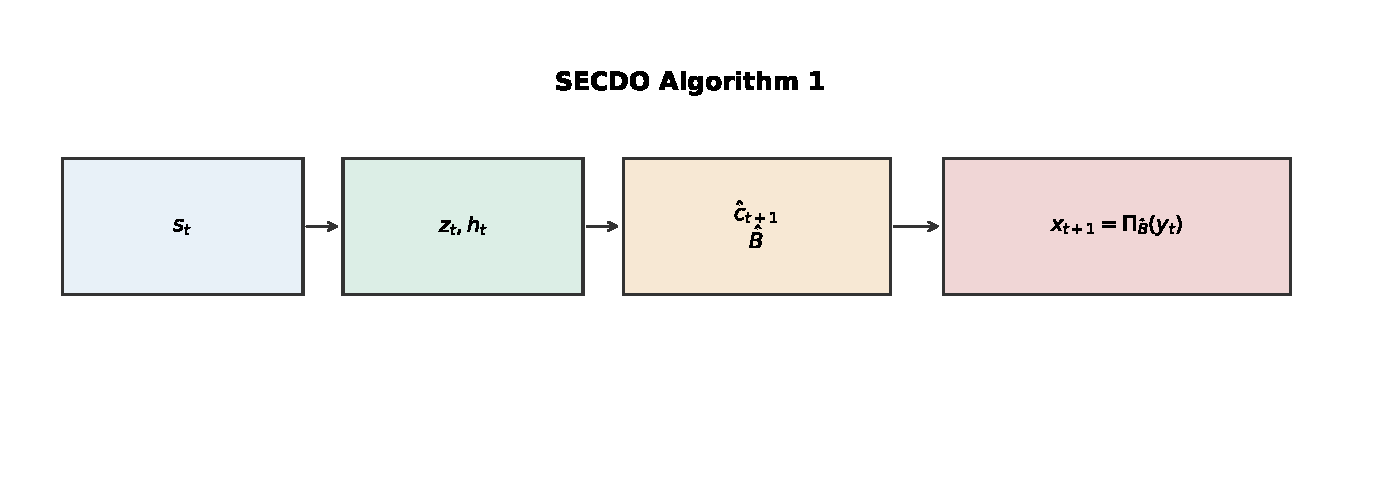
\includegraphics[width=\linewidth]{figures/fig1_framework.pdf}
\caption{SECDO loop: state encoding, constraint prediction, predictability-conditioned mixed projection.}
\label{fig:framework}
\end{figure}

\section{Problem Formulation}
\label{sec:problem}

\subsection{Static Objective, Dynamic Constraints}
At each $t$,
\begin{equation}
\min_{x\in\mathbb{R}^n} F_t(x)
\quad\text{s.t.}\quad
x\in\mathcal{B}_t=\mathcal{B}(c_t)=\{x\ge 0:\mathbf{1}^\top x\le c_t\}.
\end{equation}
Let $x_t^\star\in\arg\min_{x\in\mathcal{B}_t}F_t(x)$.
We do \emph{not} claim convergence to a moving unconstrained optimum.

\subsection{UAV Capacity Teacher}
\begin{equation}
c_t=W\log_2\bigl(1+\overline{\mathrm{SINR}}_t\bigr),\qquad
\chi_t=\lvert c_{t+1}-c_t\rvert=d_H(\mathcal{B}_{t+1},\mathcal{B}_t).
\end{equation}

\subsection{Learned Constraint Dynamics}
\begin{equation}
\hat c_{t+1}=\mathcal{F}_\phi(h_t),\qquad
\delta_t=d_H\bigl(\hat{\mathcal{B}}_{t+1},\mathcal{B}_{t+1}\bigr)
\le \lvert\hat c_{t+1}-c_{t+1}\rvert.
\end{equation}
SECDO establishes a controllable relationship between capacity residuals and feasible-set mismatch $\delta_t$---it does \emph{not} claim to learn the true future constraint exactly.

\section{Theoretical Analysis}
\label{sec:theory}

We chain five objects: constraint identifiability $\rightarrow$ projection perturbation $\rightarrow$ dynamic regret $\rightarrow$ predictability-conditioned advantage $\rightarrow$ failure-safe recovery.
Assumptions are collected in Appendix~\ref{app:impl} (cf.\ Assumps.~1--4 in the supplement markdown freeze).

\paragraph{Notation freeze.}
$\delta_t:=d_H(\hat{\mathcal{B}}_{t+1},\mathcal{B}_{t+1})$ (feasible-set mismatch);
$\chi_t:=d_H(\mathcal{B}_{t+1},\mathcal{B}_t)$ (constraint drift);
$\epsilon_t:=\|s_{t+1}-\hat s_{t+1}\|$ (state prediction error).
Capacity residual $\lvert\hat c_{t+1}-c_{t+1}\rvert$ upper-bounds $\delta_t$ for scalar budgets (Theorem~\ref{thm:1}) and is \emph{not} denoted $\delta_t$.

\subsection{Constraint Evolution Identifiability}
\begin{theorem}[Constraint evolution stability]
\label{thm:1}
For scalar budgets $\mathcal{B}(c)=\{x\ge 0:\mathbf{1}^\top x\le c\}$,
\begin{equation}
\delta_t
\;=\;
d_H\bigl(\mathcal{B}(c_{t+1}),\mathcal{B}(\hat c_{t+1})\bigr)
\;\le\;
\lvert c_{t+1}-\hat c_{t+1}\rvert.
\end{equation}
If $c=T(s)$ is $L_g$-Lipschitz and $\hat c_{t+1}=T(\hat s_{t+1})$, then
$\delta_t\le L_g\epsilon_t$.
\end{theorem}
Theorem~\ref{thm:1} establishes a controllable relationship between capacity / state residuals and feasible-set mismatch $\delta_t$, not that the predictor recovers the true future constraint.
Proof: Appendix~\ref{app:thm1}.

\begin{lemma}[Surrogate consistency]
\label{lem:surrogate}
Let $L_c=\lvert\hat c-c\rvert^2$ be the constraint regression loss and assume the scalar-budget geometry of Theorem~\ref{thm:1}.
Then
\begin{equation}
\mathbb{E}[\delta_t]
\;\le\;
\mathbb{E}\lvert\hat c_t-c_t\rvert
\;\le\;
\sqrt{\mathbb{E}[L_c]}.
\end{equation}
Hence minimizing the constraint prediction loss contracts the theoretical set-mismatch term appearing in Theorems~\ref{thm:1}--\ref{thm:2}.
This does \emph{not} claim that minimizing $L_c$ minimizes $\mathrm{Reg}_T$.
\end{lemma}
Proof: Appendix~\ref{app:surrogate}.

\subsection{Projection Error Propagation}
\begin{lemma}[Projection perturbation]
\label{lem:2}
Under bounded projection sensitivity, for any $y$,
\begin{equation}
\bigl\|\Pi_{\hat{\mathcal{B}}}(y)-\Pi_{\mathcal{B}}(y)\bigr\|
\;\le\;
C_\Pi\, d_H(\hat{\mathcal{B}},\mathcal{B}).
\end{equation}
Consequently, with $x_{t+1}=\Pi_{\hat{\mathcal{B}}_{t+1}}(y_t)$ and $x_{t+1}^\circ=\Pi_{\mathcal{B}_{t+1}}(y_t)$,
$\|x_{t+1}-x_{t+1}^\circ\|\le C_\Pi\delta_t$.
Under $\mu$-strong convexity,
$\|x_{t+1}^\star-x_t^\star\|\le\mu^{-1}(\omega_t+L_g\chi_t)$.
\end{lemma}
\begin{remark}
\label{rem:Cpi}
The constant $C_\Pi$ characterizes the sensitivity of the projection operator rather than a universal property of arbitrary convex sets.
This assumption is not required for arbitrary convex sets, but holds for the polyhedral feasible regions considered in this work; boundedness then follows from standard Hoffman-type error bounds, and often $C_\Pi=O(1)$.
\end{remark}
Proof: Appendix~\ref{app:lem2}.

\subsection{Dynamic Variational Regret}
Define $\mathrm{Reg}_T=\sum_{t=0}^{T-1}\bigl(F_t(x_t)-F_t(x_t^\star)\bigr)$ and
$P_T=\sum_{t}\|x_{t+1}^\star-x_t^\star\|$.
\begin{theorem}[Dynamic regret upper bound]
\label{thm:2}
SECDO admits a dynamic regret upper bound governed by objective drift, constraint evolution, and feasible-set mismatch:
\begin{equation}
\mathrm{Reg}_T
\;\le\;
O\Bigl(\sqrt{T(1+P_T)}\Bigr)
\;+\;
O\Bigl(\sum_t(\epsilon_t+\delta_t)\Bigr),
\end{equation}
with
\begin{equation}
P_T
\;\le\;
\frac1\mu\sum_t\bigl(\omega_t+L_g\chi_t\bigr).
\end{equation}
\end{theorem}
We do \emph{not} claim that SECDO achieves optimal regret.
Proof: Appendix~\ref{app:thm2}.

\subsection{Predictability-Conditioned Feasibility Improvement}
Let $V_R(t)\le\chi_t$ and $V_A(t)\le\delta_t$ be reactive / anticipatory future-violation certificates, and $\mathrm{PI}_t=\delta_t/(\chi_t+\varepsilon)$.
\begin{theorem}[Predictability-conditioned feasibility improvement]
\label{thm:3}
If $\mathrm{PI}_t<1$ (i.e., $\delta_t<\chi_t$), anticipatory projection provides a tighter \emph{constraint-violation certificate} when set mismatch is smaller than constraint drift:
\begin{equation}
\delta_t<\chi_t
\quad\Rightarrow\quad
\text{anticipatory feasibility certificate strictly tighter than reactive}.
\end{equation}
\end{theorem}
This is a statement about feasibility certificates, not about objective superiority, and not a claim that SECDO is always better.
Proof: Appendix~\ref{app:thm3}.

\subsection{Failure-Safe Recovery}
\begin{corollary}[Graceful degradation]
\label{cor:4}
With $\alpha_t=1/(1+\mathrm{PI}_t^2)$ and $c^{\mathrm{mix}}_t=\alpha_t\hat c_{t+1}+(1-\alpha_t)c_t$,
when $\mathrm{PI}_t\gg 1$ one has $\alpha_t\to 0$ and SECDO gracefully degrades toward reactive behavior.
Writing $I_t^{\mathrm{fail}}=\mathbf{1}\{\mathrm{PI}_t>1\}$,
\begin{equation}
\mathrm{Reg}_{\mathrm{SECDO}}
\;\le\;
\mathrm{Reg}_{\mathrm{Reactive}}
\;+\;
O\Bigl(\sum_t I_t^{\mathrm{fail}}\delta_t\Bigr).
\end{equation}
\end{corollary}
We do not claim full recovery to a failure-free trajectory.
Proof: Appendix~\ref{app:cor4}.

\section{Algorithm}
\label{sec:algo}

\begin{algorithm}[t]
\caption{SECDO with Predictively Adaptive Projection (implementation uses a continuous relaxation of the theoretical binary regimes $\alpha\in\{0,1\}$).}
\label{alg:secdo}
\begin{algorithmic}[1]
\Require step-size $\eta$; predictor $\mathcal{F}_\phi$; encoder/GRU; objective $F$
\State initialize $x_0\in\mathcal{B}(c_0)$, $h_{-1}=0$
\For{$t=0,1,\ldots,T-1$}
  \State $z_t\leftarrow\mathrm{Enc}(s_t)$,\; $h_t\leftarrow\mathrm{GRU}(z_t,h_{t-1})$
  \State $\hat s_{t+1}\leftarrow\mathrm{Dec}(h_t)$,\; $\hat c_{t+1}\leftarrow\mathcal{F}_\phi(h_t)$
  \State $y_t\leftarrow x_t-\eta\nabla F(x_t)$
  \State estimate $\hat\delta_t,\hat\chi_t$;\; $\widehat{\mathrm{PI}}_t\leftarrow\hat\delta_t/(\hat\chi_t+\varepsilon)$
  \State $\alpha_t\leftarrow 1/(1+\widehat{\mathrm{PI}}_t^2)$
  \State $c^{\mathrm{mix}}_t\leftarrow\alpha_t\hat c_{t+1}+(1-\alpha_t)c_t$
  \State $x_{t+1}\leftarrow\Pi_{\mathcal{B}(c^{\mathrm{mix}}_t)}(y_t)$
  \State observe $s_{t+1},c_{t+1}$; optional online update of $\phi$ with $\|\Delta\theta\|\le\zeta$
\EndFor
\end{algorithmic}
\end{algorithm}

\begin{remark}[Theory vs.\ implementation]
\label{rem:alpha}
The ideal anticipatory analysis in Theorems~\ref{thm:2}--\ref{thm:3} compares projections onto $\hat{\mathcal{B}}_{t+1}$ and $\mathcal{B}_t$ (extremes corresponding to $\alpha=1$ and $\alpha=0$).
The deployed Algorithm~\ref{alg:secdo} uses \emph{budget mixing} $c^{\mathrm{mix}}$ with $0<\alpha_t\le 1$, which continuously interpolates those extremes and enables Corollary~\ref{cor:4}.
The mixed feasible region preserves a \emph{single} projection operation, avoiding additional optimization overhead from combining two projected points.
Adaptive $\alpha$ is an implementation-level robustness mechanism; the core certificates characterize ideal anticipatory vs.\ reactive projection.
\end{remark}

\textbf{Training $\neq$ online algorithm.}
Offline, we minimize $L=\lambda_s L_s+\lambda_c L_c+\lambda_u L_u$ with $(\lambda_s,\lambda_c,\lambda_u)=(0.5,1.0,0.1)$.
Minimizing $L_c$ contracts $\delta$ via Lemma~\ref{lem:surrogate} but does not directly minimize $\mathrm{Reg}_T$.
During training, $\hat c$ is stop-grad through $\Pi$.
Details: Appendix~\ref{app:impl}.

\section{Experiments}
\label{sec:exp}

SECDO does not target Pareto dominance on all metrics.
We evaluate (i)~scaling structure on synthetic convex problems, (ii)~optimality--safety trade-off on UAV allocation, and (iii)~prediction-failure stress tests.

\subsection{Experimental Setup}
\textbf{Synthetic convex:} theory validation of Theorem~\ref{thm:2} scaling and PI behavior---not leaderboard tuning.
\textbf{UAV system evaluation:} practical benefit and safety/efficiency trade-off under Slow/Fast/Stress regimes (5 seeds); this demonstrates system behavior only (synthetic experiments address scaling laws).
\textbf{Prediction failure stress test:} Corollary~\ref{cor:4} via corrupted $\hat c$ windows.

\subsection{Dynamic Regret Scaling}
\begin{figure}[t]
\centering
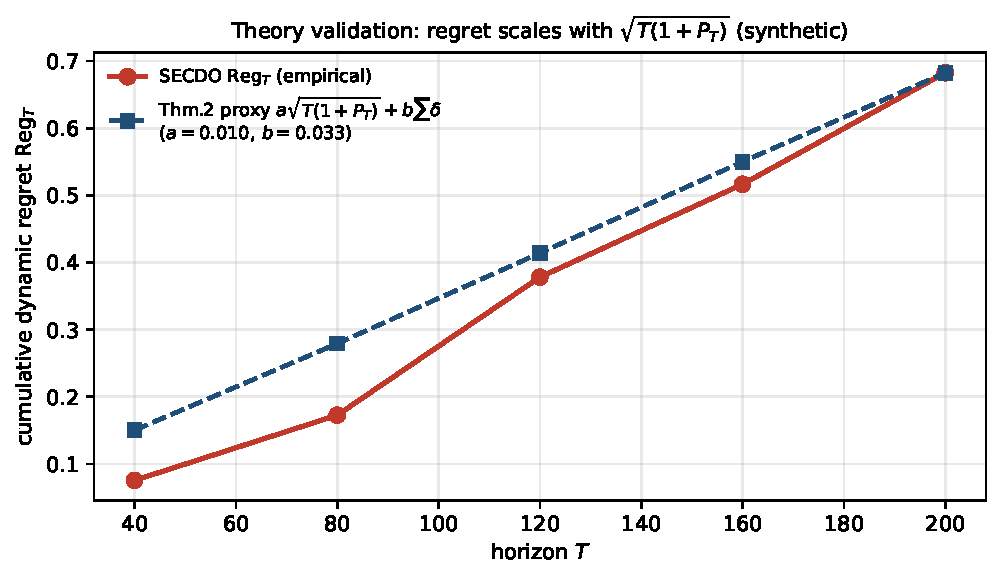
\includegraphics[width=\linewidth]{figures/fig4_regret.pdf}
\caption{Dynamic regret scaling under synthetic evolving constraints.
Empirical $\mathrm{Reg}_T$ tracks the structure $O\sqrt{T(1+P_T)}+O\sum\delta$.
The fitted envelope is only used for visualization and does not represent a universal constant.}
\label{fig:regret}
\end{figure}

Fig.~\ref{fig:regret} demonstrates the \emph{scaling behavior} predicted by Theorem~\ref{thm:2}.
Coefficients in the plotted envelope are fitted only for visualization.

\subsection{Drift Sensitivity on UAV}
\begin{table}[t]
\centering
\caption{SECDO under increasing environmental drift (5 seeds).}
\label{tab:drift}
\begin{tabular}{lccc}
\toprule
Regime & $\bar\chi$ & $\mathrm{Reg}_T$ & Violation \\
\midrule
Slow   & 0.010 & $7.69\times10^{-4}$ & 0.33\% \\
Fast   & 0.131 ($\times$13.0) & $4.36\times10^{-2}$ ($\times$56.7) & 1.46\% \\
Stress & 0.203 & $6.86\times10^{-2}$ & 1.89\% \\
\bottomrule
\end{tabular}
\end{table}
Table~\ref{tab:drift}: a $13\times$ rise in $\bar\chi$ induces a $56.7\times$ rise in $\mathrm{Reg}_T$ with bounded violation.

\subsection{Failure Recovery and PI Adaptation}
\begin{figure}[t]
\centering
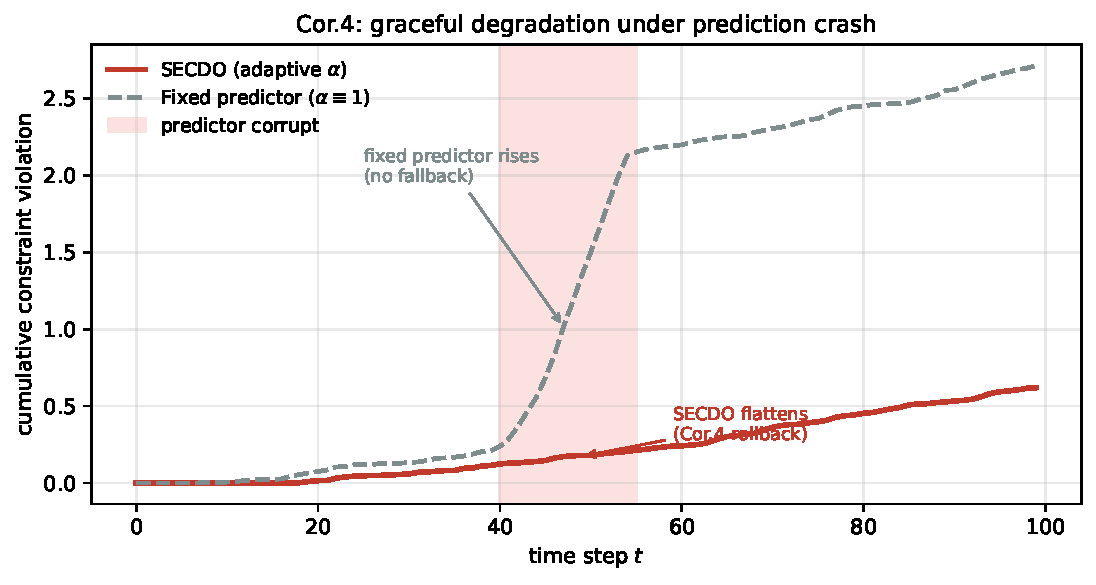
\includegraphics[width=\linewidth]{figures/fig2_crash.pdf}
\caption{Robust recovery under predictor failure (crash protocol).
SECDO gracefully degrades relative to fixed $\alpha\equiv 1$.}
\label{fig:crash}
\end{figure}
\begin{figure}[t]
\centering
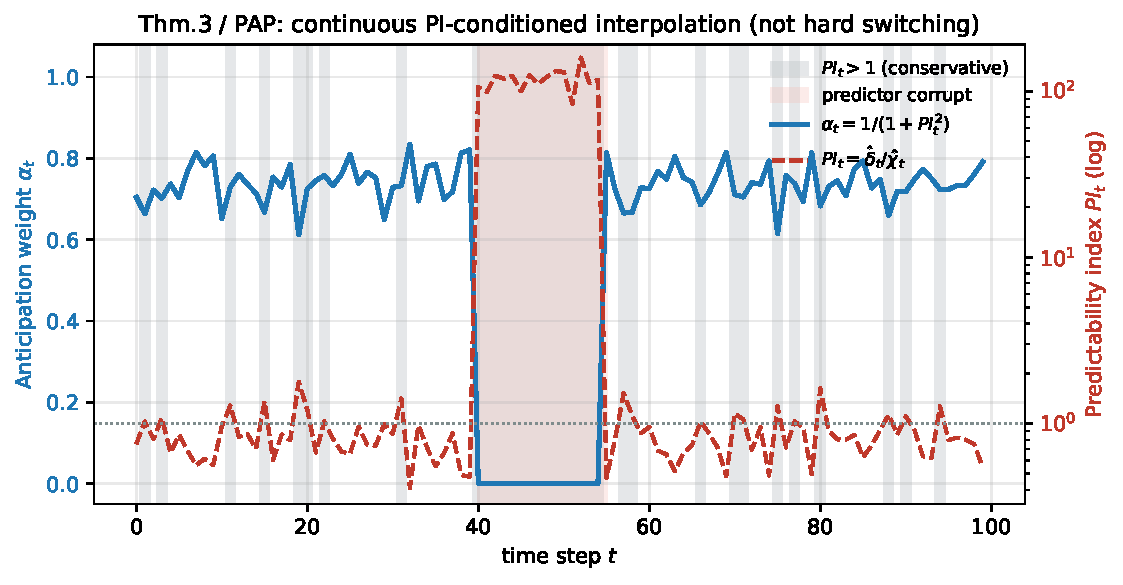
\includegraphics[width=\linewidth]{figures/fig3_PI_boundary.pdf}
\caption{Online $\mathrm{PI}_t$ and adaptive weight $\alpha_t=1/(1+\mathrm{PI}_t^2)$ under predictor corruption.}
\label{fig:pi}
\end{figure}
Figs.~\ref{fig:crash}--\ref{fig:pi} demonstrate the empirical behavior predicted by Corollary~\ref{cor:4}
and predictability-conditioned mixing.

\subsection{Optimality--Safety Trade-off}
\begin{figure}[t]
\centering
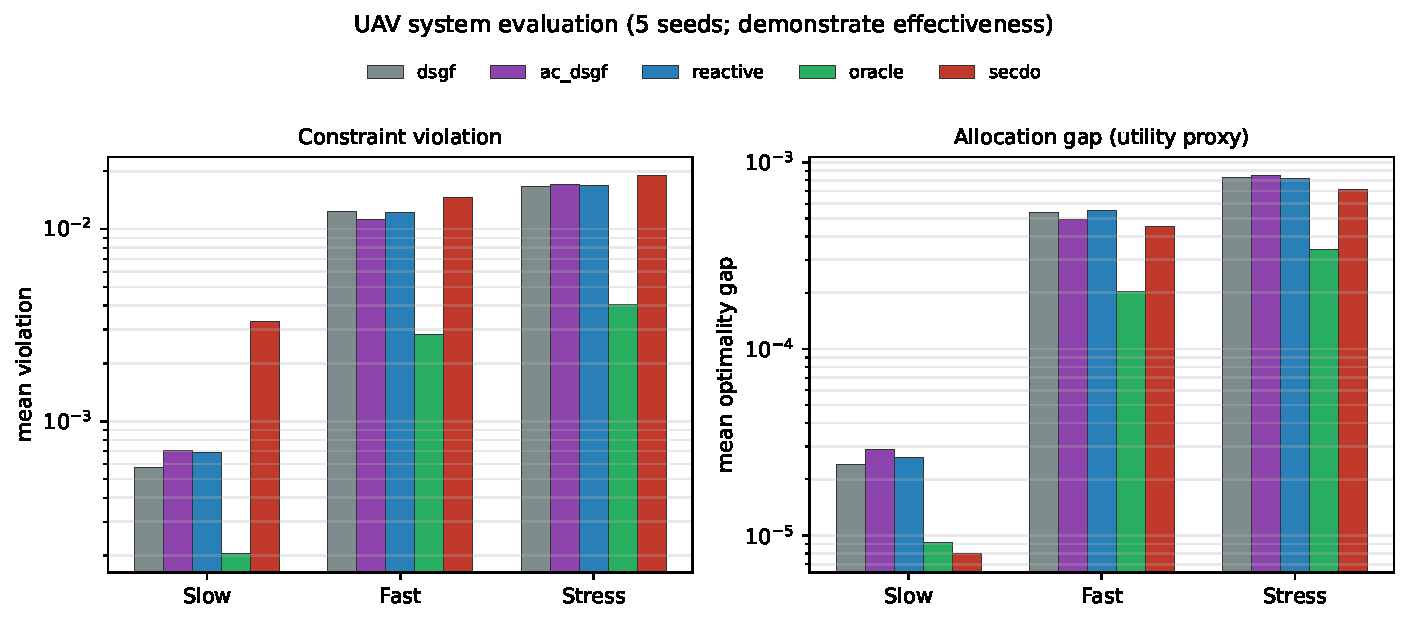
\includegraphics[width=\linewidth]{figures/fig5_uav.pdf}
\caption{Optimality--safety trade-off under dynamic constraints (UAV, 5 seeds).
SECDO achieves a favorable gap--violation trade-off relative to conservative reactive baselines.
Oracle uses future $c_{t+1}$ (informational upper bound).}
\label{fig:uav}
\end{figure}
Fig.~\ref{fig:uav}: SECDO reduces optimality gap by exploiting constraint evolution, at a moderate violation cost versus reactive methods---the expected anticipatory vs.\ conservative trade-off.

\subsection{Ablation}
\begin{table}[t]
\centering
\caption{Ablation on Fast UAV regret and crash-window cumulative-violation rise.}
\label{tab:ablation}
\begin{tabular}{lcc}
\toprule
Variant & Fast $\mathrm{Reg}_T$ & Crash window rise \\
\midrule
Full SECDO & 0.044 & 0.185 \\
A1/A2 (no anticipation) & 0.052 (+18\%) & 0.142 \\
A3 ($\alpha\equiv 1$) & 0.043 & 0.559 ($\times$3) \\
\bottomrule
\end{tabular}
\end{table}
Table~\ref{tab:ablation}: removing anticipation increases Fast regret by $\sim\!18\%$.
Adaptive $\alpha$ mainly improves robustness rather than nominal performance:
when predictions are accurate, $\alpha\equiv 1$ is nearly unchanged; under failure it prevents error amplification (Corollary~\ref{cor:4}).

\section{Conclusion}
\label{sec:concl}

SECDO is a predictive constraint-evolution framework for dynamic feasible optimization:
it learns $\hat{\mathcal{B}}_{t+1}$, applies predictability-conditioned mixed projection, and admits a dynamic regret guarantee with graceful degradation under prediction failure.
Theory (Theorems~\ref{thm:1}--\ref{thm:3}, Corollary~\ref{cor:4}), Algorithm~\ref{alg:secdo}, and experiments form a single chain---constraint evolution, anticipatory / mixed projection, adaptive robustness, and regret analysis---rather than a stack of unrelated heuristics.

\paragraph{Limitations.}
SECDO currently assumes that evolving feasible regions admit bounded projection sensitivity and focuses on online optimization with predictable constraint evolution under polyhedral (scalar-budget) geometry.
Extending the framework to highly nonconvex feasible manifolds, stronger partial observability, and fully coupled classical topology solvers remains an interesting direction.
UAV baselines for DSGF/AC-DSGF are evaluated as myopic adapters under a shared capacity teacher and should not be read as exhaustive reproductions of every historical variant.


\appendices
\section{Proof of Theorem~\ref{thm:1}}
\label{app:thm1}

Assume without loss of generality $c\ge\hat c\ge 0$. Then $\mathcal{B}(\hat c)\subseteq\mathcal{B}(c)$, so
$\sup_{z\in\mathcal{B}(\hat c)}\mathrm{dist}(z,\mathcal{B}(c))=0$.
For $x\in\mathcal{B}(c)$ with $\mathbf{1}^\top x>\hat c$, the radial map
$\tilde x=(\hat c/\mathbf{1}^\top x)\,x$ lies in $\mathcal{B}(\hat c)$ and
$\|x-\tilde x\|_2\le c-\hat c$.
Hence $d_H(\mathcal{B}(c),\mathcal{B}(\hat c))\le\lvert c-\hat c\rvert$.
The Lipschitz claim follows from Assump.~1: $\lvert T(\hat s)-T(s)\rvert\le L_g\|\hat s-s\|$.

\section{Proof of Lemma~\ref{lem:surrogate}}
\label{app:surrogate}

By Theorem~\ref{thm:1}, $\delta_t\le\lvert\hat c_t-c_t\rvert$ under scalar budgets.
Taking expectations and applying Jensen's inequality / Cauchy--Schwarz on the scalar residual yields
\begin{equation}
\mathbb{E}[\delta_t]
\;\le\;
\mathbb{E}\lvert\hat c_t-c_t\rvert
\;\le\;
\sqrt{\mathbb{E}\lvert\hat c_t-c_t\rvert^2}
\;=\;
\sqrt{\mathbb{E}[L_c]}.
\end{equation}
Thus reducing $L_c$ contracts the set-mismatch term that enters Theorems~\ref{thm:1}--\ref{thm:2}.
We emphasize that $L_c$ is a surrogate for $\delta$, not a surrogate for $\mathrm{Reg}_T$.

\section{Proof of Lemma~\ref{lem:2}}
\label{app:lem2}

By Assump.~3 (bounded projection sensitivity), for fixed $y$,
$\|\Pi_{\hat{\mathcal{B}}}(y)-\Pi_{\mathcal{B}}(y)\|\le C_\Pi d_H(\hat{\mathcal{B}},\mathcal{B})$.
Applying this at $y=y_t$ with $\hat{\mathcal{B}}=\hat{\mathcal{B}}_{t+1}$ and $\mathcal{B}=\mathcal{B}_{t+1}$ yields
$\|x_{t+1}-x_{t+1}^\circ\|\le C_\Pi\delta_t$.
The comparator motion bound follows from $\mu$-strong convexity of $F_t$ and Assump.~4 (bounded $\omega_t,\chi_t$), as in standard gradual-variation arguments for strongly convex problems.
As noted in Remark~\ref{rem:Cpi}, Assump.~3 is not claimed for arbitrary convex sets; it is used here for the polyhedral (scalar-budget) regions studied in this paper.

\section{Proof Sketch of Theorem~\ref{thm:2}}
\label{app:thm2}

Start from a projected-gradient inequality for the \emph{exact} projection onto $\mathcal{B}_{t+1}$.
Replace the exact projection by SECDO's projection onto $\hat{\mathcal{B}}_{t+1}$ (or $\mathcal{B}(c^{\mathrm{mix}})$) using Lemma~\ref{lem:2}; Lipschitz continuity of $F_t$ contributes an additive $O(\delta_t)$ term per step.
State-prediction noise in $\widehat{\nabla}_t$ contributes $O(\epsilon_t)$.
Telescope distance terms and apply the standard dynamic-regret / path-variation argument with $P_T=\sum\|x_{t+1}^\star-x_t^\star\|$, choosing $\eta\asymp\sqrt{(1+P_T)/T}$ (or an equivalent two-stage bound), to obtain
$O\sqrt{T(1+P_T)}+O\sum(\epsilon_t+\delta_t)$.
The bound on $P_T$ is Lemma~\ref{lem:2}.
Full expansions mirror the SECDO theory freeze notes (\texttt{thm2\_prediction\_aware\_gap.md}).

\section{Proof of Theorem~\ref{thm:3}}
\label{app:thm3}

For reactive $x_{t+1}^{R}=\Pi_{\mathcal{B}_t}(y_t)$,
$\mathrm{dist}(x_{t+1}^{R},\mathcal{B}_{t+1})\le d_H(\mathcal{B}_t,\mathcal{B}_{t+1})=\chi_t$,
so $V_R(t)\le\chi_t$.
For anticipatory $x_{t+1}^{A}=\Pi_{\hat{\mathcal{B}}_{t+1}}(y_t)\in\hat{\mathcal{B}}_{t+1}$,
$\mathrm{dist}(x_{t+1}^{A},\mathcal{B}_{t+1})\le\delta_t$, so $V_A(t)\le\delta_t$.
If $\delta_t<\chi_t$, the anticipatory \emph{feasibility} upper-bound certificate is strictly tighter.
This compares constraint-violation certificates, not objective superiority, and not pathwise distances on every sample.

\section{Proof Sketch of Corollary~\ref{cor:4}}
\label{app:cor4}

With $c^{\mathrm{mix}}_t=\alpha_t\hat c_{t+1}+(1-\alpha_t)c_t$ and $\alpha_t=1/(1+\mathrm{PI}_t^2)$,
\begin{equation}
\lvert c^{\mathrm{mix}}_t-c_{t+1}\rvert
\;\le\;
\alpha_t\delta_t^{\mathrm{cap}}+(1-\alpha_t)\chi_t.
\end{equation}
As $\mathrm{PI}_t\to\infty$, $\alpha_t\to 0$ and the update degrades to reactive projection onto $\mathcal{B}_t$.
Comparing per-step regret to a pure reactive baseline, excess cost on failure indicators $I_t^{\mathrm{fail}}$ is absorbed as $O(I_t^{\mathrm{fail}}\delta_t)$, yielding the stated cumulative bound.
SECDO \emph{gracefully degrades} toward reactive behavior; it does not claim full recovery.

\section{Additional Experiments}
\label{app:add}

\begin{figure}[t]
\centering
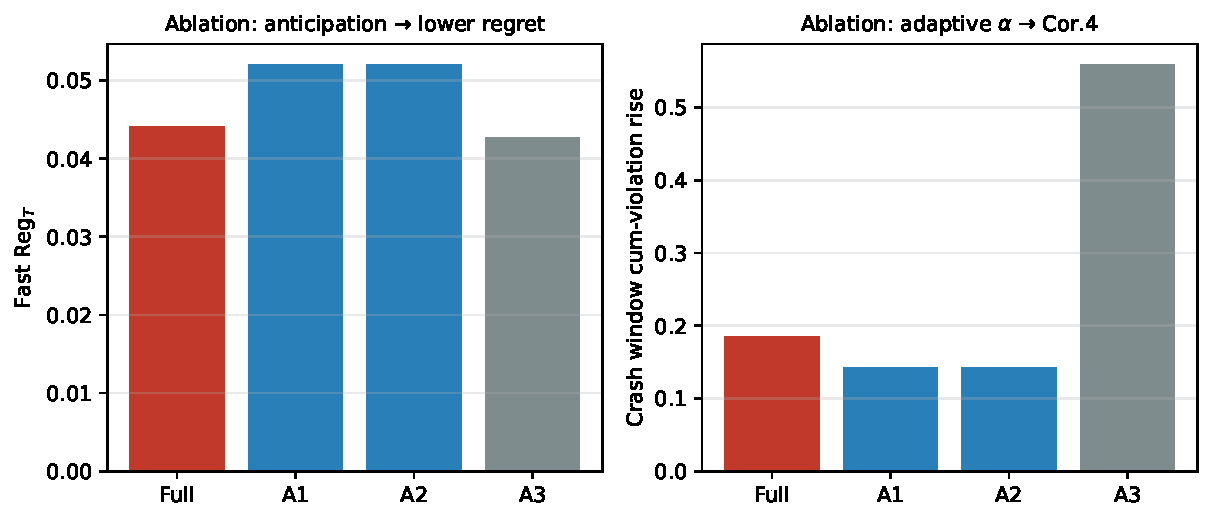
\includegraphics[width=0.9\linewidth]{figures/figE_ablation.pdf}
\caption{Ablation summary: Fast-regime regret (left) and crash-window cumulative-violation rise (right).
Demonstrates the empirical behavior predicted by Corollary~\ref{cor:4} (adaptive $\alpha$ vs.\ $\alpha\equiv 1$).}
\label{fig:ablation}
\end{figure}

Fig.~\ref{fig:ablation} expands Table~\ref{tab:ablation}.
A1/A2 coincide operationally when $\alpha=0$ (projection onto $\mathcal{B}(c_t)$).
A3 ($\alpha\equiv 1$) nearly matches Full on clean Fast UAV but inflates crash-window rise by $\approx 3\times$, isolating failure containment.

\paragraph{Evidence chain.}
Claims map to theory and figures as: Thm.~\ref{thm:1}~$\leftrightarrow\delta$ logs;
Lem.~\ref{lem:2}~$\leftrightarrow$ Oracle gap;
Thm.~\ref{thm:2}~$\leftrightarrow$ Fig.~\ref{fig:regret} \& Table~\ref{tab:drift};
Thm.~\ref{thm:3}~$\leftrightarrow$ Fig.~\ref{fig:pi};
Cor.~\ref{cor:4}~$\leftrightarrow$ Fig.~\ref{fig:crash} \& A3.

\section{Computational Complexity}
\label{app:complexity}

Let $O(P)$ denote one Euclidean projection onto a scalar-budget simplex / polytope (sorting-based, $O(n\log n)$ typical), and $O(d)$ a cheap first-order update (gradient step in allocation dimension $n$).
Let $O(C_\phi)$ be one forward pass of the constraint predictor $\mathcal{F}_\phi$.

\begin{table}[h]
\centering
\caption{Per-iteration complexity (schematic).}
\label{tab:complexity}
\begin{tabular}{lccc}
\toprule
Method & Prediction & Projection & Update \\
\midrule
Reactive & --- & $O(P)$ & $O(d)$ \\
Oracle & future $c_{t+1}$ known & $O(P)$ & $O(d)$ \\
SECDO & $O(C_\phi)$ inference & $O(P)$ (single) & $O(d)$ \\
\bottomrule
\end{tabular}
\end{table}

Relative to reactive projection, SECDO adds predictor inference $O(C_\phi)$ and scalar $\mathrm{PI}/\alpha$ arithmetic.
It does \emph{not} increase the number of projections: the mixed budget $c^{\mathrm{mix}}$ induces one set $\mathcal{B}(c^{\mathrm{mix}})$ and a single $\Pi$.
Thus prediction does not make the optimization subproblem asymptotically more expensive than reactive / oracle projection under the same geometry.

\section{Implementation Consistency}
\label{app:impl}

\paragraph{Assumptions (summary).}
Assump.~1: Lipschitz constraint/teacher map ($L_g$).
Assump.~2: $\mu$-strong convexity and $L_F$-smoothness of $F_t$.
Assump.~3: bounded projection sensitivity $C_\Pi$ (Remark~\ref{rem:Cpi}).
Assump.~4: bounded drifts $\chi_t,\omega_t$.

\paragraph{Code map.}
$\hat c$: capacity head;
$\mathrm{PI},\alpha,c^{\mathrm{mix}}$: \texttt{secdo.optimizer.secdo\_optimizer};
$\Pi$: scalar-budget projection;
$L_c$: constraint regression loss.
Oracle alone peeks $c_{t+1}$; SECDO never does.
Version tag: SECDO-v2.0; environment: conda \texttt{pytorch12}, CUDA.

\paragraph{Simplified logical chain.}
\begin{center}
\texttt{learned constraint evolution}
$\;\rightarrow\;$
\texttt{anticipatory / mixed projection}
$\;\rightarrow\;$
\texttt{adaptive robustness}
$\;\rightarrow\;$
\texttt{regret analysis}.
\end{center}
We intentionally avoid presenting PI, $\alpha$, recovery, etc.\ as independent stacked heuristics.


\bibliographystyle{IEEEtran}
% \bibliography{refs}

\end{document}
